\begin{figure}[ht]
\centering
\begin{subfigure}[t]{0.47\linewidth}
  \centering
  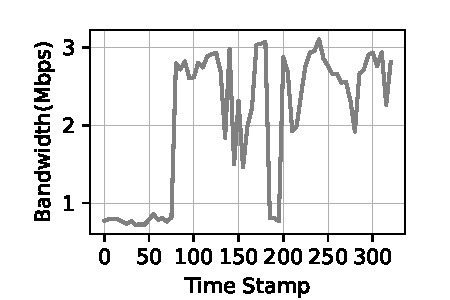
\includegraphics[width=\linewidth]{figures/chap04/evaluation_multialgo/bandwidth_68_plot.pdf}
  \caption{类型1带宽随时间变化}
  \label{type1-band-eva}
\end{subfigure}%
\begin{subfigure}[t]{0.47\linewidth}
  \centering
  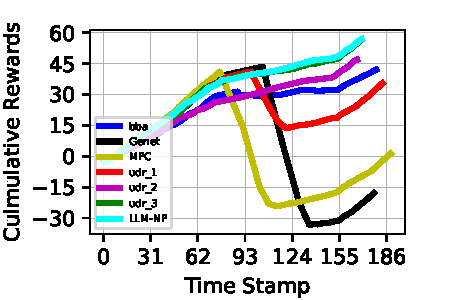
\includegraphics[width=\linewidth]{figures/chap04/evaluation_multialgo/test_68_plot.pdf}
  \caption{类型1下LLM-NP性能表现奖励值}
  \label{type1-rew-eva}
\end{subfigure}

\begin{subfigure}[t]{0.47\linewidth}
  \centering
  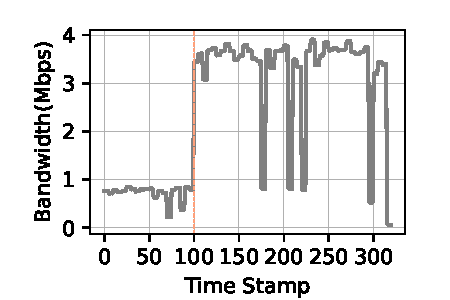
\includegraphics[width=\linewidth]{figures/chap04/evaluation_multialgo/bandwidth_27_plot.pdf}
  \caption{类型2带宽随时间变化}
  \label{type2-band-eva}
\end{subfigure}%
\begin{subfigure}[t]{0.47\linewidth}
  \centering
  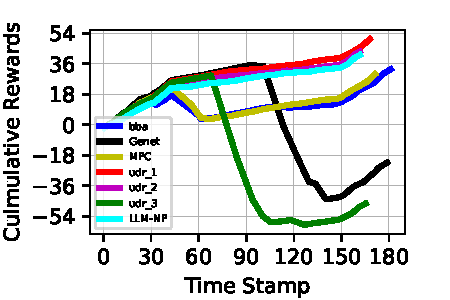
\includegraphics[width=\linewidth]{figures/chap04/evaluation_multialgo/test_27_plot.pdf}
  \caption{类型2下LLM-NP性能表现奖励值}
  \label{type2-rew-eva}
\end{subfigure}

\begin{subfigure}[t]{0.47\linewidth}
  \centering
  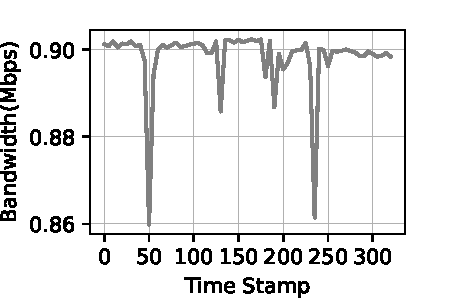
\includegraphics[width=\linewidth]{figures/chap04/evaluation_multialgo/bandwidth_88_plot.pdf}
  \caption{类型3带宽随时间变化}
  \label{type3-band-eva}
\end{subfigure}%
\begin{subfigure}[t]{0.47\linewidth}
  \centering
  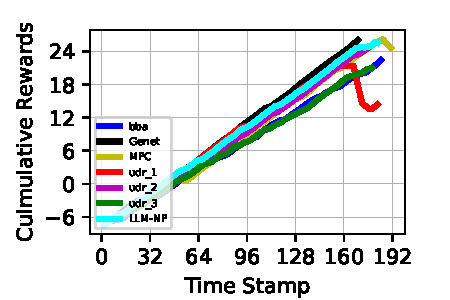
\includegraphics[width=\linewidth]{figures/chap04/evaluation_multialgo/test_88_plot.pdf}
  \caption{类型3下LLM-NP性能表现奖励值}
  \label{type3-rew-eva}
\end{subfigure}

\caption{三个类型网络环境下LLM-NP与传统算法的奖励值对比}
\label{fig:multi-algo-eva}
\end{figure}
